\documentclass[a4paper,12pt]{report}
\usepackage[utf8]{inputenc}
\usepackage[T1,T2A]{fontenc}
\usepackage[english,russian]{babel}
\usepackage{amsfonts}
\usepackage{amsmath}
\usepackage{upgreek}
\usepackage{amssymb}
\usepackage{wasysym}
\usepackage{graphicx}
\usepackage{amsthm}
\usepackage{hyperref}
\usepackage{geometry}
\usepackage{listings}
\usepackage{xcolor}

% Настройка геометрии страницы
\geometry{left=3cm, right=1.5cm, top=2cm, bottom=2cm}

% Настройка hyperref
\hypersetup{
    colorlinks=true,
    linkcolor=blue,
    filecolor=magenta,      
    urlcolor=cyan,
    citecolor=blue
}

% Настройка листингов кода
\lstset{
    basicstyle=\ttfamily\small,
    keywordstyle=\color{blue},
    commentstyle=\color{green},
    stringstyle=\color{red},
    showstringspaces=false,
    breaklines=true,
    frame=single,
    numbers=left,
    numberstyle=\tiny\color{gray}
}

\title{Проект по случайным графам}
\author{Ильин Павел, Кулешов Илья, ПАДИИ, 2 курс}
\date{\today}

\begin{document}

\maketitle

\tableofcontents

% ===== ВВЕДЕНИЕ =====
\chapter*{Введение}
\addcontentsline{toc}{chapter}{Введение}

Данный отчёт описывает исследование свойств случайных графов, построенных на основе различных вероятностных распределений. В работе рассматриваются два типа графов: графы k-ближайших соседей (KNN) и дистанционные графы.

\textbf{Цель работы:} Исследовать поведение числовых характеристик случайных графов в зависимости от параметров распределений и параметров построения графов.

\textbf{Задачи:}
\begin{enumerate}
    \item Исследовать поведение числа треугольников, минимального кликового числа, числа компонент и хроматического числа в зависимости от параметров распределений
    \item Исследовать влияние параметров процедуры построения графа и размера выборки
    \item Построить статистические и ML критерии и оценить их мощность
\end{enumerate}

% ===== ЧАСТЬ 1 =====
\part{Исследование свойств характеристик графов}

\chapter{Исследование поведения числовой характеристики $\tau$ в зависимости от параметров распределений}

\section{Методология исследования}

\subsection{Описание числовых характеристик}
В работе исследуются 4 основные характеристики:
\begin{itemize}
    \item $\tau^{KNN}$ - количество треугольников в графе k-ближайших соседей
    \item $\tau^{dist}$ - минимального кликовое число дистанционного графа
    \item $\tau^{KNN}$ - количество компонент связности в графе k-ближайших соседей
    \item $\tau^{dist}$ - хроматическое число дистанционного графа
\end{itemize}

\subsection{Исследуемые распределения}
\textbf{Эксперимент 1:} Normal vs Student-t
\begin{itemize}
    \item Нормальное распределение $N(0, \alpha)$
    \item Распределение Стьюдента с $\nu$ степенями свободы
\end{itemize}

\textbf{Эксперимент 2:} Pareto vs Gamma
\begin{itemize}
    \item Распределение Парето с параметром $\alpha$
    \item Гамма-распределение с параметрами shape и scale
\end{itemize}

\subsection{Применяемые ML алгоритмы}
\begin{itemize}
    \item Логистическая регрессия
    \item Решающее дерево
    \item Градиентный бустинг (CatBoost) с iterations = 50
\end{itemize}

\subsection{Разное техническое}
\begin{itemize}
    \item Все замеры проводятся методом Монте-Карло с 20 итерациями (кроме тех случаев, когда явно будет указано другое число) 
    \item Базовое количество соседей для графа KNN - 5
    \item Базовое расстояние в дистанционном графе - 1.0
    \item Так как подсчет минимального кликового покрытия, подсчет хроматического числа - NP полные задачи, их вычисление происходит с помощью Python библиотеки networkx жадными методами. 
    \item Для минимального кликового покрытия для удобства запускается подсчет хроматического числа дополнения графа (ввиду равенства данных величин)

\end{itemize}

\section{Характеристики графов при различных параметрах распределений}

\subsection{Эксперимент 1: Normal vs Student-t}

На графике ниже видно, что параметры распределения не влияют никак на KNN граф, однако в dist графе наблюдается монотонная тенденция для каждого распределения

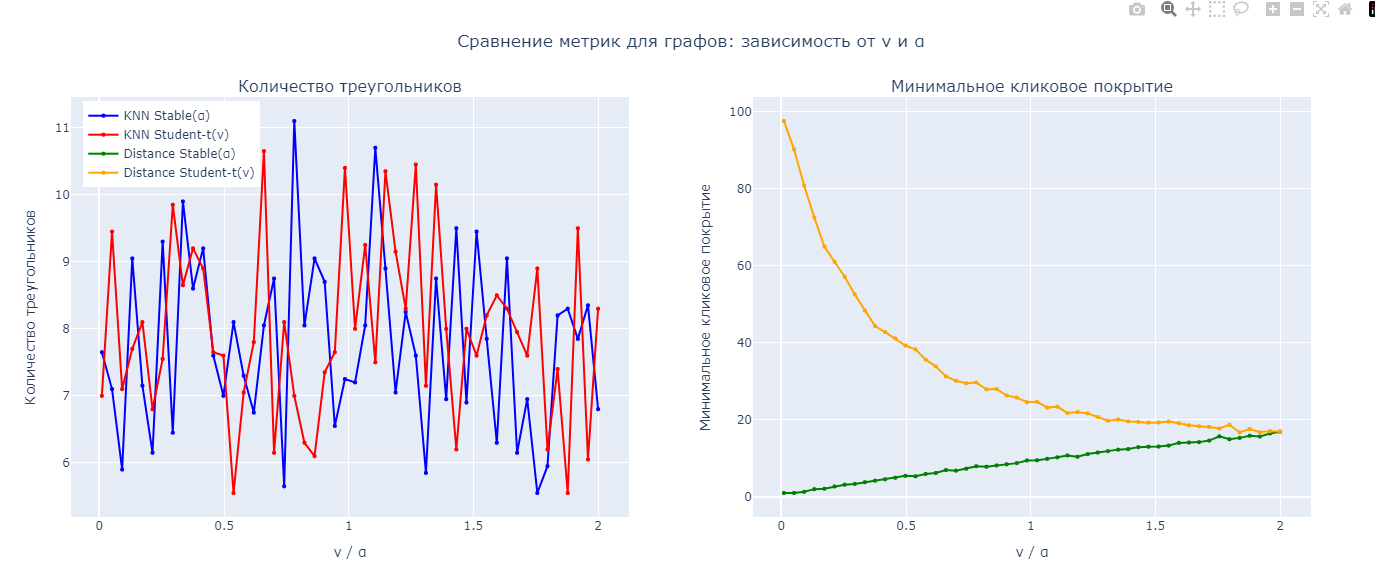
\includegraphics[width=1\linewidth]{images/ilin_part1.png}

\subsection{Эксперимент 2: Pareto vs Gamma}

На графике ниже видно, что число компонент почти всегда - 1, однако в dist графе наблюдается монотонная тенденция для каждого распределения, но в различные стороны
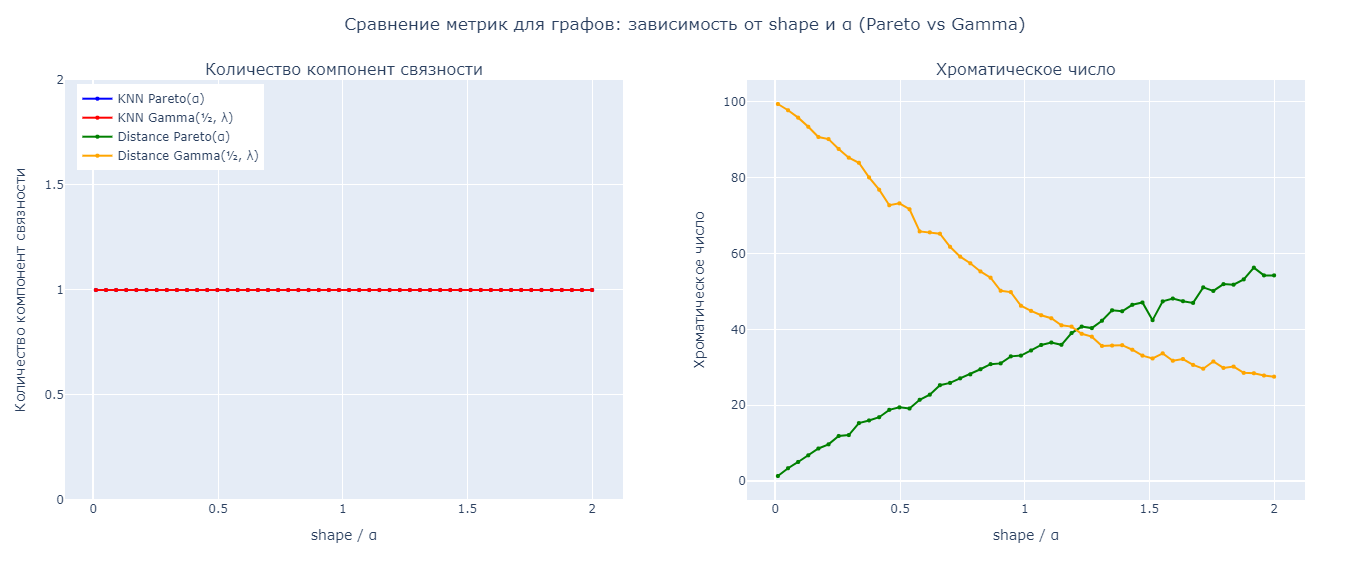
\includegraphics[width=1\linewidth]{images/kuleshov_part1.png}

\chapter{Исследование поведения характеристики $\tau$ в зависимости от параметров построения графа}

\section{Эксперимент 1: Normal vs Student-t}

Рассмотрим для начала число треугольников в KNN-графе: при увеличении n и k количество треугольников в каждом распределении увеличивается - в целом это логично (больше граф - больше ребер - больше треугольников). В случае дистанцинного графа, кликовое число растет вместе с n, но уменьшается с ростом d (тоже логично - больше ребер - меньше клик нужно).


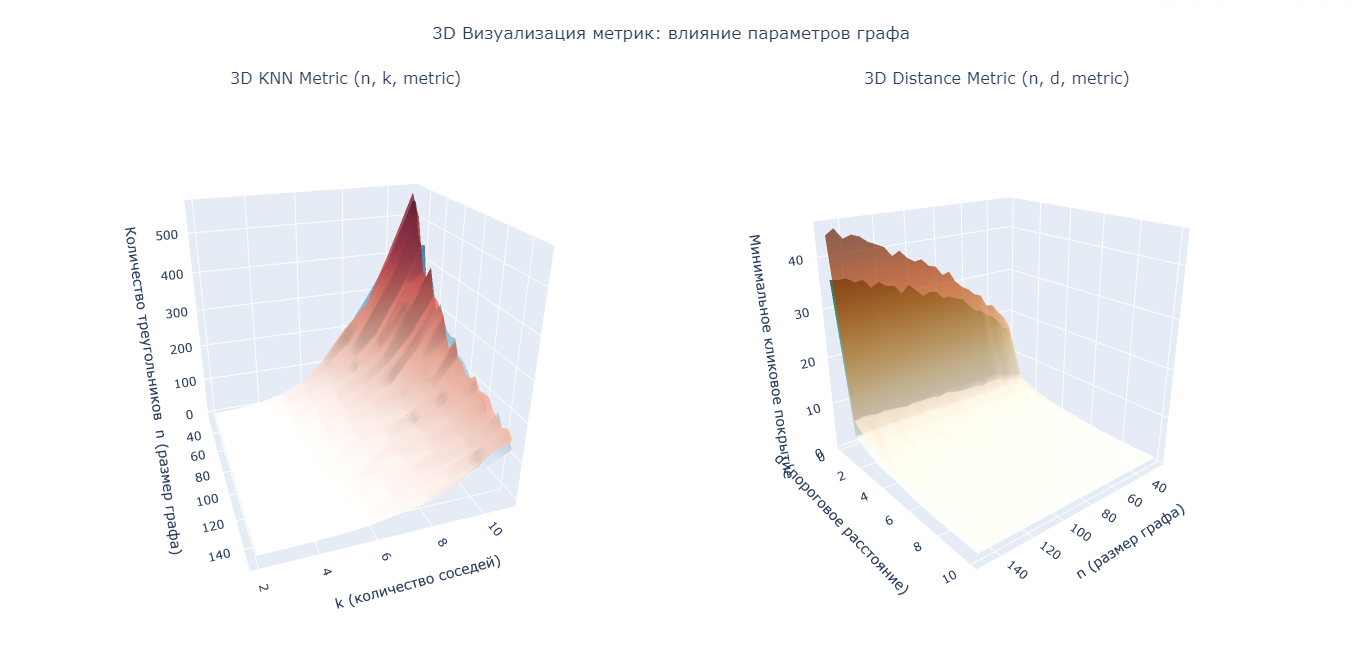
\includegraphics[width=1\linewidth]{images/ilin_part2.png}

\section{Эксперимент 2: Pareto vs Gamma}

Видно, что число компонент связности почти всегда 1 при различных n и парамерах построения KNN-графа, однако бывают и небольшие выбросы иногда. Для хроматического числа все поинтереснее - при минимальных d нам достаточно пары цветов (так как граф разряжен), но в среднем с ростом n и уменьшением d наблюдается тенденция на рост хроматического числа

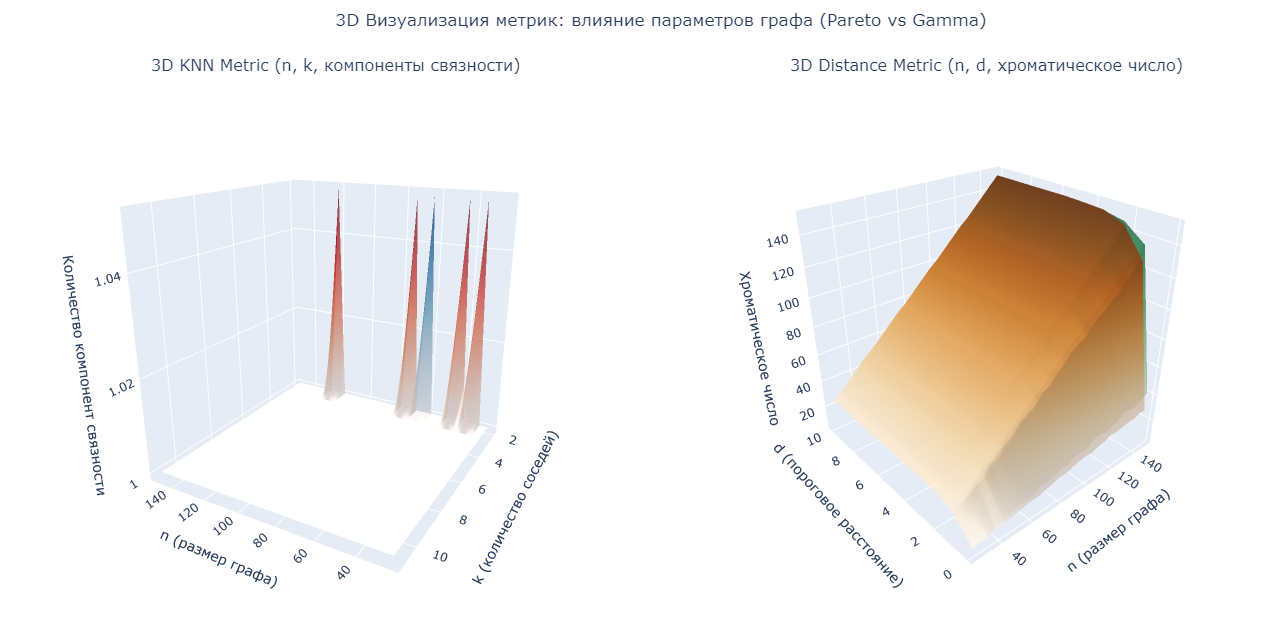
\includegraphics[width=1\linewidth]{images/kuleshov_part2.png}

\chapter{Построение статистических критериев}

\section{Критерии для Normal и Student-t}

\subsection{Построение множества A при $\alpha = 0.05$}

Для подсчета статистического критерия разбиения используется 500 итераций метода Монте-Карло для формирования выборок, а затем взятие 95-го перцентиля плотности f (Normal и Pareto соответственно) для минимизации ошибки первого рода

\subsection{Оценка мощности критерия для Normal и Student-t}

Видно, что для KNN графа и его характеристики сложно выбрать хороший критерий в целом. Однако для дистанционного графа Student-t и Normal сильно различаются по своим средним, что позволяет критерию для минимизации ошибки первого рода быть в целом качественным критерием.

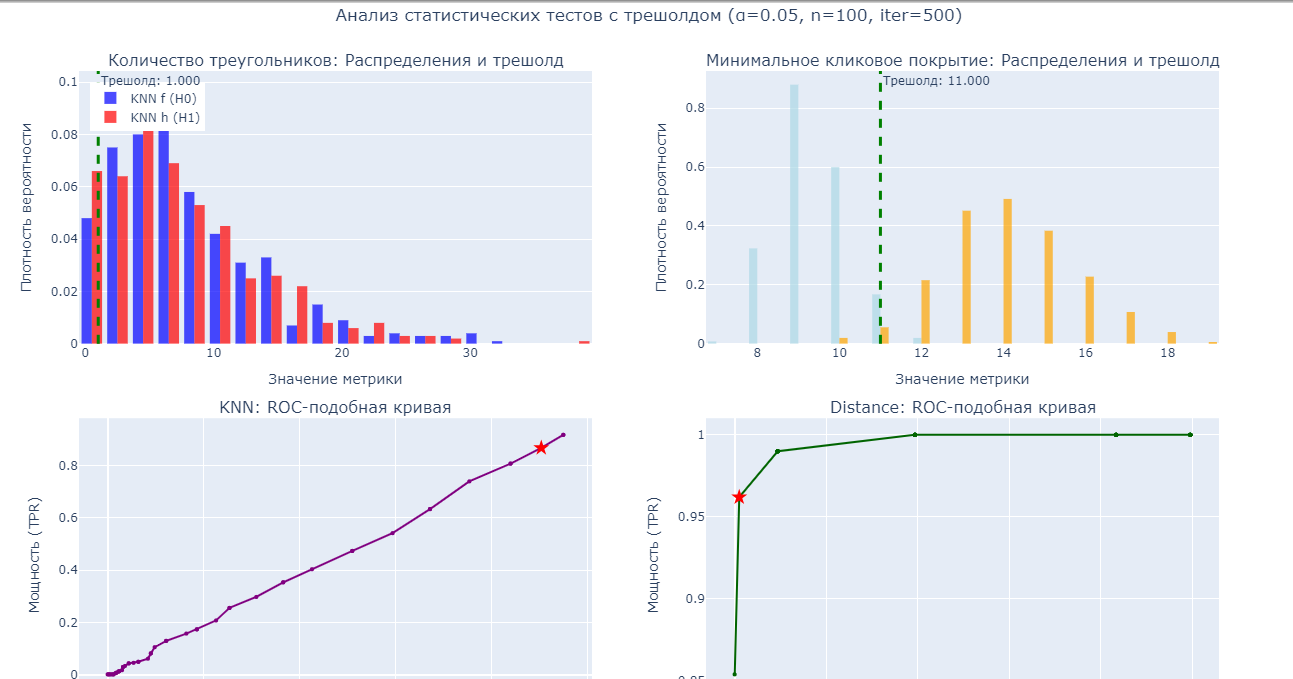
\includegraphics[width=1\linewidth]{images/ilin_part3.png}
\subsection{Оценка мощности критерия для Pareto и Gamma}

Видно, что для KNN графа и его характеристики сложно выбрать хороший критерий в целом. Однако для дистанционного графа Student-t и Normal сильно различаются по своим средним, что позволяет критерию для минимизации ошибки первого рода быть в целом качественным критерием.

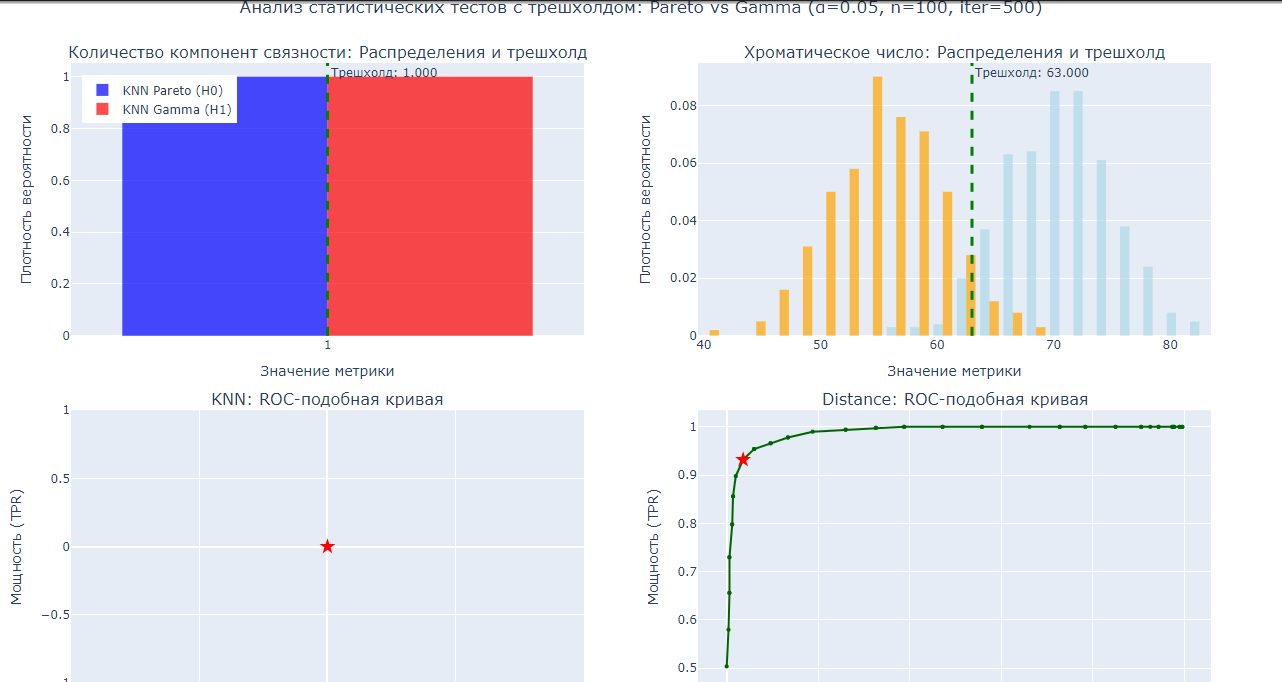
\includegraphics[width=1\linewidth]{images/kuleshov_part3.png}

% ===== ЧАСТЬ 2 =====
\part{Применение машинного обучения для классификации распределений}

\chapter{Классификация с использованием нескольких характеристик}

\section{Подготовка данных}

\subsection{Формирование датасетов}
Для генерации датасетов были выбраны размеры графа : n = [25, 100, 500], затем с помощью 50 итераций метода Монте-Карло формировались наблюдения вида [размер графа, параметр построения, характеристика, тип распределения]. 

Для анализа был взят дистанционный граф.

\section{Эксперимент 1: Normal vs Student-t}

\subsection{Результаты для различных размеров графов}

В целом лучше всего себя показал градиентный бустинг CatBoost (подписан как ctb). Линейная модель не смогла грамотно оценить зависимость по такому малому количеству данных, а решающее дерево просто средне обучилось.

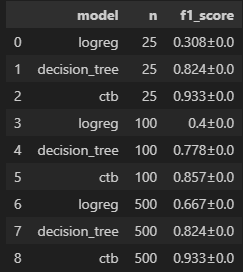
\includegraphics[width=0.5\linewidth]{images/ilin_part4.png}

\subsection{Оценка мощности критерия по ML}

Несмотря на неплохие показатели f1-score, который является средним гармоническим для ошибок первого и второго рода, сам критерий ошибки первого рода не получился достаточно качественным 

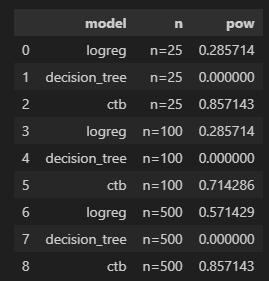
\includegraphics[width=0.5\linewidth]{images/ilin_part5.png}

\section{Эксперимент 2: Pareto vs Gamma}

\subsection{Результаты для различных размеров графов}

В целом лучше всего себя показал градиентный бустинг CatBoost (подписан как ctb), хотя в среднем модели получили чуть худшее качество, чем в предыдущем эскперимете

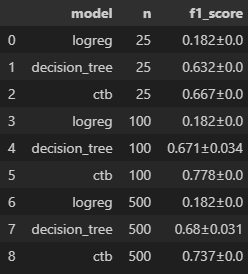
\includegraphics[width=0.5\linewidth]{images/kuleshov_part4.png}

\subsection{Оценка мощности критерия по ML}

Несмотря на ухудшение качества общего, мощность критерия в лучшем случае осталась неизменной относительно предыдущего эксперимента

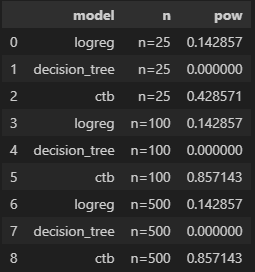
\includegraphics[width=0.5\linewidth]{images/kuleshov_part5.png}


% ===== ЗАКЛЮЧЕНИЕ =====
\chapter*{Заключение}
\addcontentsline{toc}{chapter}{Заключение}

\section*{Основные результаты}
Мы исследовали поведение 4 различных характеристик для двух типов графов в различных распределениях и определили различные критерии для оценки принадлежности графа к какому либо типу (по исходному распределению). 

\subsection{KNN}
Для KNN графов распределения были не так важны - и это понятно, ведь для каждой вершины мы берем всегда k ближайших соседей и неважно как они далеко, поэтому есть гипотеза, что действительно критичным для KNN графа является не просто само распределение, а локальные различия в изменениях плотности - так например при подсчете треугольников для KNN графа равномерного распределения будут в среднем получатся последовательные клики размера k, а в распределениях с явными пиками, в этих пиках вполне могут получаться клики размера 2k (если достаточно точек было изначально). Если же распределения локально имеют различные виды участков, (Student-t и Normal), то граф будет слишком случайным по количеству треугольников (что было видно выше на картинке). Аналогично для подсчета числа компонент (только тут все еще менее интересно)

\subsection{Dist}

Для дистанционных графов все интереснее, чем для KNN, ведь здесь на различные характеристики графа влияет уже не только изменение плотности, но и среднее и дисперсия распределения. Ввиду этого можно наблюдать различное поведение. Также графическим меодом было доказано, что минимальное кликовое число графа можно считать через хроматическое число дополнения графа. (3D график хроматического числа инвертировать по n и d и получим график минимального кликового покрытия). 
В конечном итоге, именно большая динамичность и большая случайность таких графов, позволяют качественно разделять различные исходные распределения между собой даже в одномерном случае, в отличие от KNN

% ===== БИБЛИОГРАФИЯ =====
\begin{thebibliography}{99}

\bibitem{networkx} NetworkX developers. NetworkX: Network Analysis in Python. \url{https://networkx.org/}

\bibitem{sklearn} Scikit-learn developers. Scikit-learn: Machine Learning in Python. \url{https://scikit-learn.org/}

\bibitem{catboost} CatBoost developers. CatBoost: Gradient Boosting on Decision Trees. \url{https://catboost.ai/}

\bibitem{numpy} NumPy developers. NumPy: The fundamental package for scientific computing with Python. \url{https://numpy.org/}

\end{thebibliography}

\end{document}